\section{Design and Implementation}
The development of the web application went through a lot of ideas before settling on the current choice of technologies used. The application uses the JavaScript library React for the frontend and user interface, and the Python web framework Flask for the backend algorithms. The initial designs, choices made and features implemented are expanded on below.

\subsection{Software Requirements}
Before any software was written, a list of requirements for the software was made. These are features that the software must have in order to fulfill the relevant objectives, and were subsequently tested throughout the development of the web application:
\begin{enumerate}
    \item Allow a user to enter Dyck words.
    \item Validate a given input and provide a relevant error message if required.
    \item Display the given Dyck word with the ability for manual interaction via a mouse.
    \item Verify that the characters selected are a valid move before allowing them to be paired.
    \item Allow for the use of strategies from literature (Simple, Non-Simple recursive), as well as our own strategies (Simple Greedy, Brute Force).
    \item If selecting a strategy, generate a list of moves before visualising the play.
    \item Display the list of moves, and allow the user to jump to any move in the play.
    \item Display a running width counter from the moves seen so far, and the width of the overall play if a strategy has been used.
    % \item (OPTIONAL) Allow for a mix between manual re-pairing and the use of pre-defined strategies (e.g. re-pairing the first half of a word using a strategy, and completing the second half using manual selections).
    \item Allow the user to brute force a given list of Dyck Words, and return the optimal widths of each along with the re-pairing.
\end{enumerate}

\subsection{Initial Ideas}

The project was initially to be a local Python only application, using Tkinter. This was because the author is most familiar with the Python programming language, and has some limited experience with the Tkinter library. However, early prototypes of this software using Tkinter proved to be cumbersome to work with and have a dated visual style. Alternative Python UI libraries (such as PyQt and Kivy) were also considered, but proved to have learning curves no steeper than using an entirely different language.
\begin{figure}[H]
    \centering
    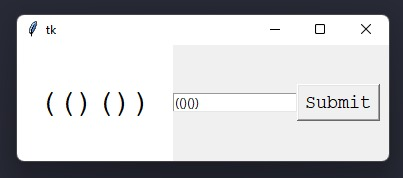
\includegraphics[scale = 0.7]{./images/tkinter-gui.jpeg}
    \caption{An early iteration of the software using Tkinter}
\end{figure}
\noindent We then turned our attention to the prospect of a web application; the author again had some limited experience with HTML/CSS but using these languages to control the layout and sizing of the UI seemed much more intuitive. This approach also naturally allowed for separation between the UI and the strategies, and the author's familiarity with Python could still be leveraged as a backend language. The author had also wished to learn the technologies used for web development, so this seemed like the natural approach to take.

\subsection{Strategy Implementation}
The strategies to run on Dyck words were implemented in Python, and communicated with the UI using Flask. This is a web framework that allows users to build a web server with python that they can communicate with using http requests, allowing Python to be used as a backend language \cite{whatisFlask}. 

\par\null\par
\noindent One of the reasons Flask was chosen over potential alternatives such as Django is due to its simplicity. Flask is classed as a microframework, meaning it does not have a lot of dependencies or libraries required to use it. This makes Flask fairly lightweight and efficient for our purposes, reducing overhead when communicating requests back and forth. 

\begin{figure}[H]
    \centering
    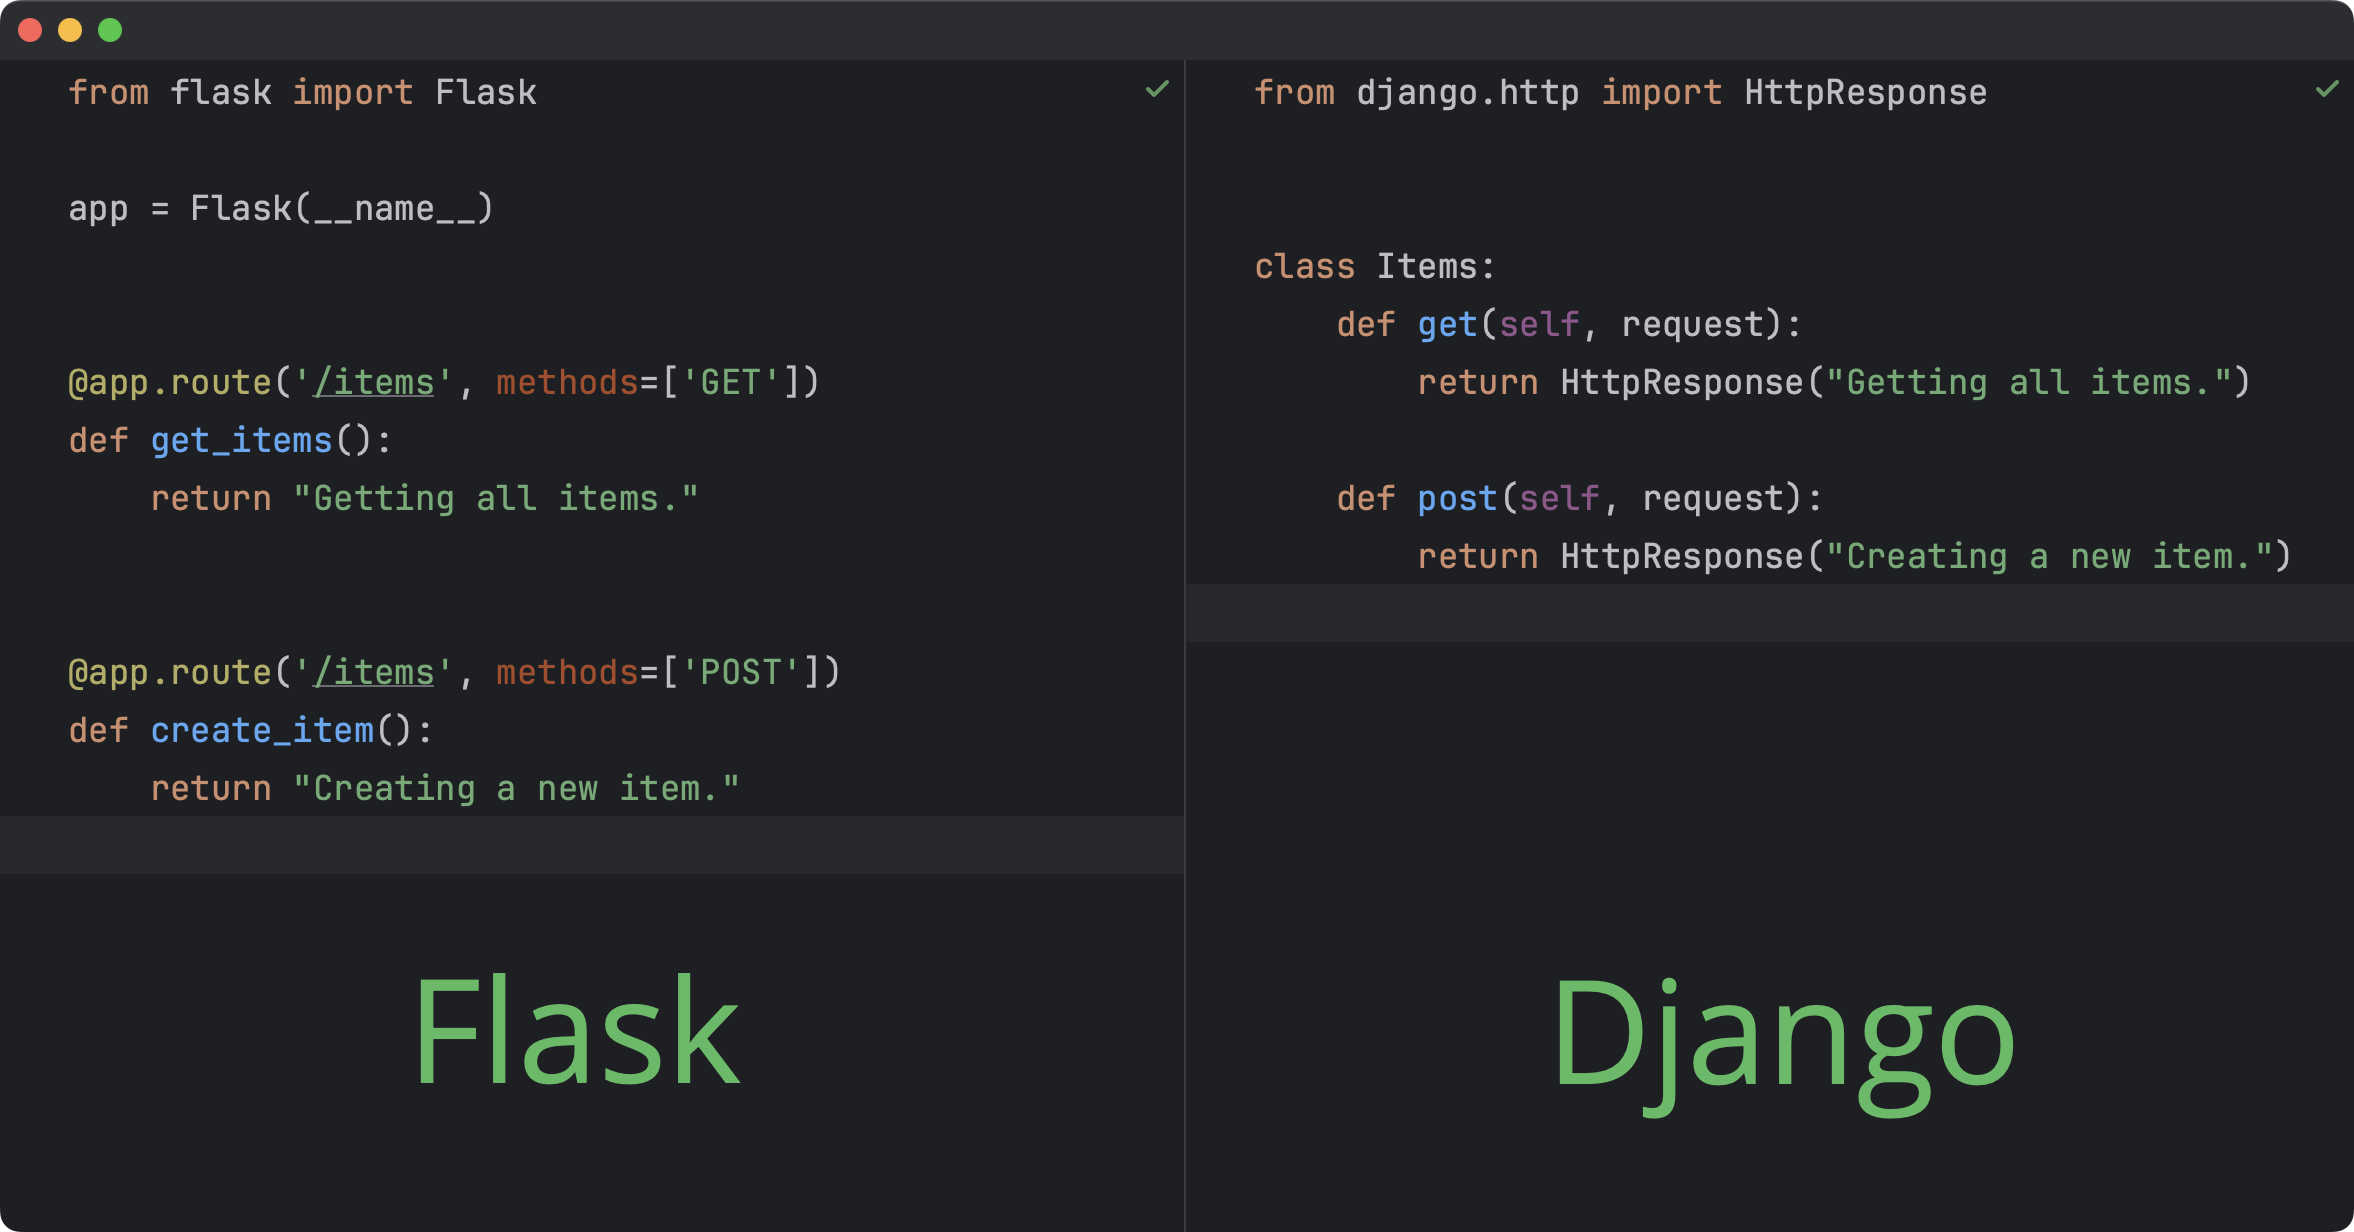
\includegraphics[scale=0.3]{./images/flaskVSdjango.png}
    \caption{Implementing the same functionality in Flask and Django \cite{flaskVSdjango}}
\end{figure}

\noindent Figure 3.2 shows the difference between using Flask and Django. In the Flask example, the same functions could be used as is once an app route is added above. This binds each function to the route URL plus its given route, and depending on the type of request either ``get\textunderscore~items()'' or \\ \noindent``create\textunderscore~items()'' would be called. Thus, any work done to translate a re-pairing strategy into an algorithm could easily be implemented using Flask by simply adding an app route at the top.

\par\null\par
\noindent Below we will outline the algorithms written from each strategy. The process of then translating this into Python is trivial.

\subsection{UI Implementation}
\noindent If a web-application was to be used, the components of the UI would need ways of interacting with one another. This led to using React, which is a JavaScript library used to simplify the process of creating user interfaces \cite{whatisReact}. It allows modular user interface components to be built, and later nested and combined to create a dynamic and interactive webpage. 

\par\null\par
\noindent The web application is designed as a single page application (SPA), meaning it loads only a single web document and updates its contents dynamically. In contrast, typical websites will make the web browser load entire new pages when the contents of the page need to be modified \cite{singlepageapp}. React fits the development of SPAs well, since each component has its own state and properties, and React will only automatically re-render components if there is a change to one of these.
This allows for greater performance gains and a more dynamic experience.

\par\null\par
\noindent Rather than styling the components of the web application from scratch, the author opted to use Material UI. This is a React component library that implements the design language made by Google, and contains a collection of prebuilt components with customisation options.

\begin{figure}[H]
    \centering
    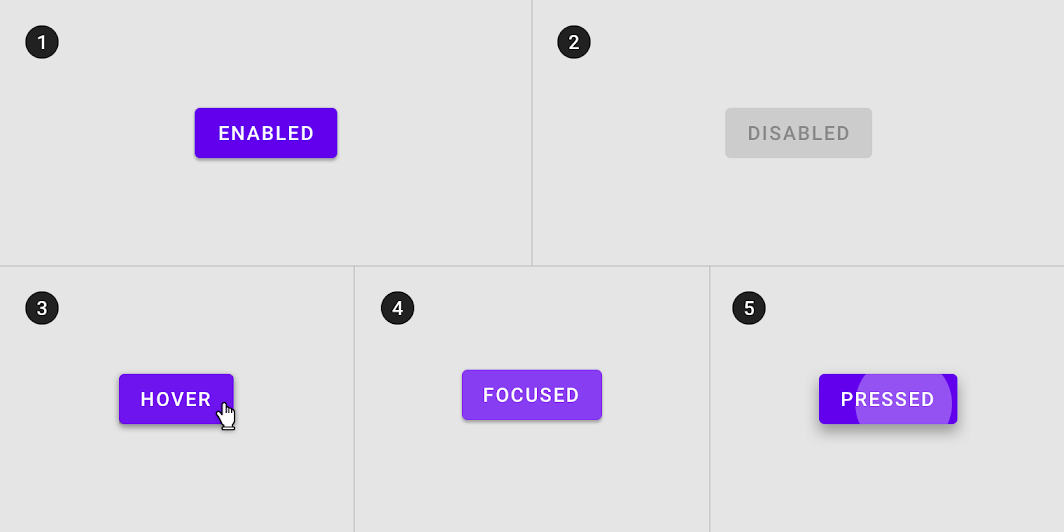
\includegraphics[scale=0.3]{./images/materialUIbutton.png}
    \caption{An example of how a Material UI button varies depending on its state}
\end{figure}

\par\null\par
\noindent We elaborate on the different parts of the UI, and how they were implemented below.

\subsubsection{Submission Box}